\documentclass[]{article}
\usepackage{lmodern}
\usepackage{amssymb,amsmath}
\usepackage{ifxetex,ifluatex}
\usepackage{fixltx2e} % provides \textsubscript
\ifnum 0\ifxetex 1\fi\ifluatex 1\fi=0 % if pdftex
  \usepackage[T1]{fontenc}
  \usepackage[utf8]{inputenc}
\else % if luatex or xelatex
  \ifxetex
    \usepackage{mathspec}
    \usepackage{xltxtra,xunicode}
  \else
    \usepackage{fontspec}
  \fi
  \defaultfontfeatures{Mapping=tex-text,Scale=MatchLowercase}
  \newcommand{\euro}{€}
\fi
% use upquote if available, for straight quotes in verbatim environments
\IfFileExists{upquote.sty}{\usepackage{upquote}}{}
% use microtype if available
\IfFileExists{microtype.sty}{\usepackage{microtype}}{}
\usepackage[margin=1in]{geometry}
\usepackage{color}
\usepackage{fancyvrb}
\newcommand{\VerbBar}{|}
\newcommand{\VERB}{\Verb[commandchars=\\\{\}]}
\DefineVerbatimEnvironment{Highlighting}{Verbatim}{commandchars=\\\{\}}
% Add ',fontsize=\small' for more characters per line
\newenvironment{Shaded}{}{}
\newcommand{\AlertTok}[1]{\textcolor[rgb]{1.00,0.00,0.00}{\textbf{#1}}}
\newcommand{\AnnotationTok}[1]{\textcolor[rgb]{0.38,0.63,0.69}{\textbf{\textit{#1}}}}
\newcommand{\AttributeTok}[1]{\textcolor[rgb]{0.49,0.56,0.16}{#1}}
\newcommand{\BaseNTok}[1]{\textcolor[rgb]{0.25,0.63,0.44}{#1}}
\newcommand{\BuiltInTok}[1]{#1}
\newcommand{\CharTok}[1]{\textcolor[rgb]{0.25,0.44,0.63}{#1}}
\newcommand{\CommentTok}[1]{\textcolor[rgb]{0.38,0.63,0.69}{\textit{#1}}}
\newcommand{\CommentVarTok}[1]{\textcolor[rgb]{0.38,0.63,0.69}{\textbf{\textit{#1}}}}
\newcommand{\ConstantTok}[1]{\textcolor[rgb]{0.53,0.00,0.00}{#1}}
\newcommand{\ControlFlowTok}[1]{\textcolor[rgb]{0.00,0.44,0.13}{\textbf{#1}}}
\newcommand{\DataTypeTok}[1]{\textcolor[rgb]{0.56,0.13,0.00}{#1}}
\newcommand{\DecValTok}[1]{\textcolor[rgb]{0.25,0.63,0.44}{#1}}
\newcommand{\DocumentationTok}[1]{\textcolor[rgb]{0.73,0.13,0.13}{\textit{#1}}}
\newcommand{\ErrorTok}[1]{\textcolor[rgb]{1.00,0.00,0.00}{\textbf{#1}}}
\newcommand{\ExtensionTok}[1]{#1}
\newcommand{\FloatTok}[1]{\textcolor[rgb]{0.25,0.63,0.44}{#1}}
\newcommand{\FunctionTok}[1]{\textcolor[rgb]{0.02,0.16,0.49}{#1}}
\newcommand{\ImportTok}[1]{#1}
\newcommand{\InformationTok}[1]{\textcolor[rgb]{0.38,0.63,0.69}{\textbf{\textit{#1}}}}
\newcommand{\KeywordTok}[1]{\textcolor[rgb]{0.00,0.44,0.13}{\textbf{#1}}}
\newcommand{\NormalTok}[1]{#1}
\newcommand{\OperatorTok}[1]{\textcolor[rgb]{0.40,0.40,0.40}{#1}}
\newcommand{\OtherTok}[1]{\textcolor[rgb]{0.00,0.44,0.13}{#1}}
\newcommand{\PreprocessorTok}[1]{\textcolor[rgb]{0.74,0.48,0.00}{#1}}
\newcommand{\RegionMarkerTok}[1]{#1}
\newcommand{\SpecialCharTok}[1]{\textcolor[rgb]{0.25,0.44,0.63}{#1}}
\newcommand{\SpecialStringTok}[1]{\textcolor[rgb]{0.73,0.40,0.53}{#1}}
\newcommand{\StringTok}[1]{\textcolor[rgb]{0.25,0.44,0.63}{#1}}
\newcommand{\VariableTok}[1]{\textcolor[rgb]{0.10,0.09,0.49}{#1}}
\newcommand{\VerbatimStringTok}[1]{\textcolor[rgb]{0.25,0.44,0.63}{#1}}
\newcommand{\WarningTok}[1]{\textcolor[rgb]{0.38,0.63,0.69}{\textbf{\textit{#1}}}}
\usepackage{graphicx}
\makeatletter
\def\maxwidth{\ifdim\Gin@nat@width>\linewidth\linewidth\else\Gin@nat@width\fi}
\def\maxheight{\ifdim\Gin@nat@height>\textheight\textheight\else\Gin@nat@height\fi}
\makeatother
% Scale images if necessary, so that they will not overflow the page
% margins by default, and it is still possible to overwrite the defaults
% using explicit options in \includegraphics[width, height, ...]{}
\setkeys{Gin}{width=\maxwidth,height=\maxheight,keepaspectratio}
\ifxetex
  \usepackage[setpagesize=false, % page size defined by xetex
              unicode=false, % unicode breaks when used with xetex
              xetex]{hyperref}
\else
  \usepackage[unicode=true]{hyperref}
\fi
\hypersetup{breaklinks=true,
            bookmarks=true,
            pdfauthor={Justin Le},
            pdftitle={A (Dead End?) Arrowized Dataflow Parallelism Interface Attempt},
            colorlinks=true,
            citecolor=blue,
            urlcolor=blue,
            linkcolor=magenta,
            pdfborder={0 0 0}}
\urlstyle{same}  % don't use monospace font for urls
% Make links footnotes instead of hotlinks:
\renewcommand{\href}[2]{#2\footnote{\url{#1}}}
\setlength{\parindent}{0pt}
\setlength{\parskip}{6pt plus 2pt minus 1pt}
\setlength{\emergencystretch}{3em}  % prevent overfull lines
\setcounter{secnumdepth}{0}

\title{A (Dead End?) Arrowized Dataflow Parallelism Interface Attempt}
\author{Justin Le}
\date{April 3, 2014}

\begin{document}
\maketitle

\emph{Originally posted on
\textbf{\href{https://blog.jle.im/entry/a-dead-end-arrowized-dataflow-parallelism-interface-attempt.html}{in
Code}}.}

So I've been having several `dead end' projects in Haskell recently that I've
sort of just scrapped and move from, but I decided that it might be nice to
document some of them :) For reading back on it later, for people to possibly
help/offer suggestions, for people to peruse and possibly learn something, or
for people to laugh at me. Here is my most recent semi-failure --- implicit
dataflow parallelism through an Arrow interface.

tl;dr:

\begin{enumerate}
\def\labelenumi{\arabic{enumi}.}
\tightlist
\item
  Compose parallelizable computations using expressive proc notation.
\item
  Consolidate and join forks to maintain maximum parallelization.
\item
  All data dependencies implicit; allows for nice succinct direct translations
  of normal functions.
\item
  All ``parallelizable'' functions can also trivially be typechecked and run as
  normal functions, due to arrow polymorphism.
\end{enumerate}

The main problem:

\begin{itemize}
\tightlist
\item
  Consider \texttt{ParArrow\ a\ c}, \texttt{ParArrow\ b\ d},
  \texttt{ParArrow\ (c,d)\ (e,f)}, \texttt{ParArrow\ e\ g}, and
  \texttt{ParArrow\ f\ h}. We execute the first two in parallel, apply the
  third, and execute the second two in parallel. Basically, we want two
  independent \texttt{ParArrow\ a\ g} and \texttt{ParArrow\ c\ h} that we can
  fork. And this is possible, as long as the ``middle'' arrow does not
  ``cross-talk'' --- that is, it can't be something like
  \texttt{arr\ (\textbackslash{}(x,y)\ -\textgreater{}\ (y,x))}.
\end{itemize}

\hypertarget{the-vision}{%
\section{The Vision}\label{the-vision}}

So what do I mean?

\hypertarget{dataflow-parallelism}{%
\subsection{Dataflow Parallelism}\label{dataflow-parallelism}}

By ``dataflow parallelism'', I refer to structuring parallel computations by
``what depends on what''. If two values \emph{can} be computed in parallel, then
that is taken advantage of. Consider something like \texttt{map\ f\ xs}.
Normally, this would: one by one step over \texttt{xs} and apply \texttt{f} to
each one, building a new list as you go along one at a time.

But note that there are some easy places to parallelize this --- because none of
the results the mapped list depend on each other, you can apply \texttt{f} to
every element in parallel, and re-collect everything back at the end. And this
is a big deal if \texttt{f} takes a long time. This is an example of something
commonly referred to as ``embarrassingly parallel''.

\hypertarget{arrows}{%
\subsection{Arrows}\label{arrows}}

So what kind of Arrow interface am I imagining with this?

Haskell has some nice syntax for composing ``functions'' (\texttt{f},
\texttt{g}, and \texttt{h}):

\begin{Shaded}
\begin{Highlighting}[]
\NormalTok{proc x }\OtherTok{{-}>} \KeywordTok{do}
\NormalTok{    y }\OtherTok{<{-}}\NormalTok{ f }\OperatorTok{{-}<}\NormalTok{ x}
\NormalTok{    z }\OtherTok{<{-}}\NormalTok{ g }\OperatorTok{{-}<}\NormalTok{ x}
\NormalTok{    q }\OtherTok{<{-}}\NormalTok{ h }\OperatorTok{{-}<}\NormalTok{ y}
\NormalTok{    returnA }\OperatorTok{{-}<}\NormalTok{ y }\OperatorTok{*}\NormalTok{ z }\OperatorTok{+}\NormalTok{ q}
\end{Highlighting}
\end{Shaded}

A \texttt{proc} statement is a fancy lambda, which takes an input \texttt{x} and
``funnels'' \texttt{x} through several different ``functions'' --- in our case,
\texttt{f}, \texttt{g}, and \texttt{h} --- and lets you name the results so that
you can use them later.

\begin{figure}
\centering
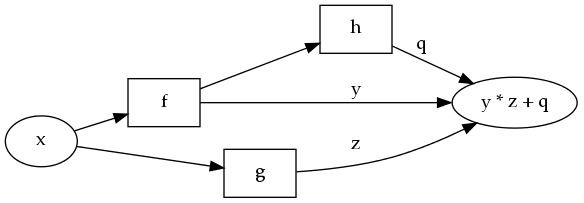
\includegraphics{/img/entries/pararrow/proc1.png}
\caption{The above proc statement, diagrammed.}
\end{figure}

While this looks like you are `performing' \texttt{f}, then \texttt{g}, then
\texttt{h}, what is actually happening is that you are \emph{composing} and
synthesizing a \emph{new function}. You are ``assembling'' a new function that,
when given an \texttt{x}, collects the results of \texttt{x} run through
\texttt{f}, \texttt{g}, and \texttt{h}, and pops out a function of what comes
out of those functions.

Except\ldots{}\texttt{f}, \texttt{g}, and \texttt{h} don't have to be normal
functions. They are ``generalized'' functions; functions that could perhaps even
have side-effects, or trigger special things, or be evaluated in special ways.
They are instances of the \texttt{Arrow} typeclass.

An \texttt{Arrow\ a\ b} just represents, abstractly, a way to get some
\texttt{b} from some \texttt{a}, equipped with combinators that allow you to
compose them in neat ways. Proc notation allows us to assemble a giant new
arrow, from sequencing and composing smaller arrows.

\hypertarget{forking-arrows}{%
\subsection{Forking Arrows}\label{forking-arrows}}

Look at the proc statement and tell me that that doesn't scream ``data
parallelism'' to you. Because every arrow \texttt{f}, \texttt{g}, and \texttt{h}
can potentially do side-effecty, stateful, IO things, depending on how we
implemented the arrow\ldots what if \texttt{f}, \texttt{g}, and \texttt{h}
represented ``a way to get a \texttt{b} from an \texttt{a}\ldots in its own
separate thread''?

So if I were to ``run'' this special arrow, a \texttt{ParArrow\ a\ b}, I would
do

\begin{Shaded}
\begin{Highlighting}[]
\OtherTok{runPar ::} \DataTypeTok{ParArrow}\NormalTok{ a b }\OtherTok{{-}>}\NormalTok{ a }\OtherTok{{-}>} \DataTypeTok{IO}\NormalTok{ b}
\end{Highlighting}
\end{Shaded}

Where if i gave \texttt{runPar} a \texttt{ParArrow\ a\ b}, and an \texttt{a}, It
would fork itself into its own thread and give you an \texttt{IO\ b} in response
to your \texttt{a}.

Because of Arrow's ability to ``separate out'' and ``side-chain'' compositions
(note that \texttt{q} in the previous example does not depend on \texttt{z} at
all, and can clearly be launched in parallel alongside the calculation of
\texttt{z}), it looks like from a \texttt{proc} notation statement, we can
easily write arrows that all `fork themselves' under composition.

Using this, in the above proc example with the fancy diagram, we should be able
to see that \texttt{z} is completely independent of \texttt{y} and \texttt{q},
so the \texttt{g} arrow could really compute itself ``in parallel'', forked-off,
from the \texttt{f} and \texttt{h} arrows.

You should also be able to ``join together'' parallel computations. That is, if
you have an \texttt{a\ -\textgreater{}\ c} and a \texttt{b\ -\textgreater{}\ d},
you could make a ``parallel'' \texttt{(a,b)\ -\textgreater{}\ (c,d)}. But what
if I also had a \texttt{c\ -\textgreater{}\ e} and a
\texttt{d\ -\textgreater{}\ f}? I could chain the entire
\texttt{a}-\texttt{c}-\texttt{e} chain and the \texttt{b}-\texttt{d}-\texttt{f}
chain, and perform both chains in parallel and re-collect things at the end.
That is, a \texttt{(a,b)\ -\textgreater{}\ (c,d)} and a
\texttt{(c,d)\ -\textgreater{}\ (e,f)} should meaningfully compose into a
\texttt{(a,b)\ -\textgreater{}\ (e,f)}, where the left and right sides (the
\texttt{a\ -\textgreater{}\ e} and the \texttt{b\ -\textgreater{}\ f}) are
performed ``in parallel'' from each other.

With that in mind, we could even do something like \texttt{parMap}:

\begin{Shaded}
\begin{Highlighting}[]
\OtherTok{parMap ::} \DataTypeTok{ParArrow}\NormalTok{ a b }\OtherTok{{-}>} \DataTypeTok{ParArrow}\NormalTok{ [a] [b]}
\NormalTok{parMap f }\OtherTok{=}\NormalTok{ proc input }\OtherTok{{-}>} \KeywordTok{do}
    \KeywordTok{case}\NormalTok{ input }\KeywordTok{of}
\NormalTok{      []     }\OtherTok{{-}>}
\NormalTok{          returnA        }\OperatorTok{{-}<}\NormalTok{ []}
\NormalTok{      (x}\OperatorTok{:}\NormalTok{xs) }\OtherTok{{-}>} \KeywordTok{do}
\NormalTok{          y  }\OtherTok{<{-}}\NormalTok{ f        }\OperatorTok{{-}<}\NormalTok{ x}
\NormalTok{          ys }\OtherTok{<{-}}\NormalTok{ parMap f }\OperatorTok{{-}<}\NormalTok{ xs}
\NormalTok{          returnA        }\OperatorTok{{-}<}\NormalTok{ y}\OperatorTok{:}\NormalTok{ys}
\end{Highlighting}
\end{Shaded}

And because ``what depends on what'' is so \emph{obviously clear} from proc/do
notation --- you know exactly what depends on what, and the graph is already
laid out there for you --- and because \texttt{f} is actually a ``smart''
function, with ``smart'' semantics which can do things like fork threads to
solve itself\ldots this should be great way to structure programs and take
advantage of implicit data parallelism.

\hypertarget{the-coolest-thing}{%
\subsubsection{The coolest thing}\label{the-coolest-thing}}

Also notice something cool -- if leave our proc blocks polymorphic:

\begin{Shaded}
\begin{Highlighting}[]
\OtherTok{map\textquotesingle{} ::} \DataTypeTok{ArrowChoice}\NormalTok{ r }\OtherTok{=>}\NormalTok{ r a b }\OtherTok{{-}>}\NormalTok{ r [a] [b]}
\NormalTok{map\textquotesingle{} f }\OtherTok{=}\NormalTok{ proc input }\OtherTok{{-}>} \KeywordTok{do}
    \KeywordTok{case}\NormalTok{ input }\KeywordTok{of}
\NormalTok{      []     }\OtherTok{{-}>}
\NormalTok{          returnA        }\OperatorTok{{-}<}\NormalTok{ []}
\NormalTok{      (x}\OperatorTok{:}\NormalTok{xs) }\OtherTok{{-}>} \KeywordTok{do}
\NormalTok{          y  }\OtherTok{<{-}}\NormalTok{ f        }\OperatorTok{{-}<}\NormalTok{ x}
\NormalTok{          ys }\OtherTok{<{-}}\NormalTok{ map\textquotesingle{} f   }\OperatorTok{{-}<}\NormalTok{ xs}
\NormalTok{          returnA        }\OperatorTok{{-}<}\NormalTok{ y}\OperatorTok{:}\NormalTok{ys}
\end{Highlighting}
\end{Shaded}

We can now use \texttt{map\textquotesingle{}} as \emph{both} a normal,
sequential function \emph{and} a parallel, forked computation!

\begin{Shaded}
\begin{Highlighting}[]
\NormalTok{λ}\OperatorTok{:}\NormalTok{          map\textquotesingle{} (arr (}\OperatorTok{*}\DecValTok{2}\NormalTok{)) [}\DecValTok{1}\OperatorTok{..}\DecValTok{5}\NormalTok{]}
\NormalTok{[}\DecValTok{2}\NormalTok{,}\DecValTok{4}\NormalTok{,}\DecValTok{6}\NormalTok{,}\DecValTok{8}\NormalTok{,}\DecValTok{10}\NormalTok{]}
\NormalTok{λ}\OperatorTok{:}\NormalTok{ runPar }\OperatorTok{$}\NormalTok{ map\textquotesingle{} (arr (}\OperatorTok{*}\DecValTok{2}\NormalTok{)) [}\DecValTok{1}\OperatorTok{..}\DecValTok{5}\NormalTok{]}
\NormalTok{[}\DecValTok{2}\NormalTok{,}\DecValTok{4}\NormalTok{,}\DecValTok{6}\NormalTok{,}\DecValTok{8}\NormalTok{,}\DecValTok{10}\NormalTok{]}
\end{Highlighting}
\end{Shaded}

Yup!

Let's try implementing it, and let's see where things go wrong.

\hypertarget{pararrow}{%
\section{ParArrow}\label{pararrow}}

\hypertarget{data-and-instances}{%
\subsection{Data and Instances}\label{data-and-instances}}

Let's start out with our arrow data type:

\begin{Shaded}
\begin{Highlighting}[]
\CommentTok{{-}{-} source: https://github.com/mstksg/inCode/tree/master/code{-}samples/pararrow/ParArrow.hs\#L12{-}L18}

\KeywordTok{data} \DataTypeTok{ParArrow}\NormalTok{ a b }\OtherTok{=}                     \DataTypeTok{Pure}\NormalTok{  (a }\OtherTok{{-}>}\NormalTok{ b)}
                  \OperatorTok{|} \KeywordTok{forall}\NormalTok{ z}\OperatorTok{.}           \DataTypeTok{Seq}\NormalTok{   (}\DataTypeTok{ParArrow}\NormalTok{ a z)}
\NormalTok{                                              (}\DataTypeTok{ParArrow}\NormalTok{ z b)}
                  \OperatorTok{|} \KeywordTok{forall}\NormalTok{ a1 a2 b1 b2}\OperatorTok{.} \DataTypeTok{Par}\NormalTok{   (a }\OtherTok{{-}>}\NormalTok{ (a1, a2))}
\NormalTok{                                              (}\DataTypeTok{ParArrow}\NormalTok{ a1 b1)}
\NormalTok{                                              (}\DataTypeTok{ParArrow}\NormalTok{ a2 b2)}
\NormalTok{                                              ((b1, b2) }\OtherTok{{-}>}\NormalTok{ b)}
\end{Highlighting}
\end{Shaded}

So a \texttt{ParArrow\ a\ b} represents a (pure) paralleizable, forkable
computation that returns a \texttt{b} (as \texttt{IO\ b}) when given an
\texttt{a}.\footnote{Technically, all \texttt{ParArrow} computations are pure,
  so you might not loose too much by just returning a \texttt{b} instead of an
  \texttt{IO\ b} with \texttt{unsafePerformIO}, but\ldots{}}

\begin{itemize}
\item
  \texttt{Pure\ f} wraps a pure function in a \texttt{ParArrow} that computes
  that function in a fork when necessary.
\item
  \texttt{Seq\ f\ g} sequences a \texttt{ParArrow\ a\ z} and a
  \texttt{ParArrow\ z\ b} into a big \texttt{ParArrow\ a\ b}. It represents
  composing two forkable functions into one big forkable function, sequentially.
\item
  \texttt{Par\ l\ f\ g\ r} takes two \texttt{ParArrow}s \texttt{f} and
  \texttt{g} of different types and represents the idea of performing them in
  parallel. Of forking them off from each other and computing them
  independently, and collecting it all together.

  \texttt{l} and \texttt{r} are supposed to be functions that turn the tupled
  inputs/outputs of the parallel computations and makes them fit
  \texttt{ParArrow\ a\ b}. \texttt{r} is kind of supposed to be \texttt{id}, and
  \texttt{l} is supposed to be \texttt{id} (to continue a parallel action) or
  \texttt{\textbackslash{}x\ -\textgreater{}\ (x,x)} (to begin a fork).

  It's a little hacky, and there might be a better way with GADT's and all sorts
  of type/kind-level magic, but it was the way I found that I understood the
  most.

  The main purpose of \texttt{l} and \texttt{r} is to be able to meaningfully
  refer to the two parallel \texttt{ParArrow}s in terms of the \texttt{a} and
  \texttt{b} of the ``combined'' \texttt{ParArrow}. Otherwise, the two inputs of
  the two parallel \texttt{ParArrow}s don't have anything to do with the input
  type \texttt{a} of the combined \texttt{ParArrow}, and same for output.
\end{itemize}

Okay, let's define a Category instance, that lets us compose \texttt{ParArrow}s:

\begin{Shaded}
\begin{Highlighting}[]
\CommentTok{{-}{-} source: https://github.com/mstksg/inCode/tree/master/code{-}samples/pararrow/ParArrow.hs\#L20{-}L22}

\KeywordTok{instance} \DataTypeTok{Category} \DataTypeTok{ParArrow} \KeywordTok{where}
    \FunctionTok{id}    \OtherTok{=} \DataTypeTok{Pure} \FunctionTok{id}
\NormalTok{    f }\OperatorTok{.}\NormalTok{ g }\OtherTok{=} \DataTypeTok{Seq}\NormalTok{ g f}
\end{Highlighting}
\end{Shaded}

No surprises there, hopefully! Now an Arrow instance:

\begin{Shaded}
\begin{Highlighting}[]
\CommentTok{{-}{-} source: https://github.com/mstksg/inCode/tree/master/code{-}samples/pararrow/ParArrow.hs\#L24{-}L29}

\KeywordTok{instance} \DataTypeTok{Arrow} \DataTypeTok{ParArrow} \KeywordTok{where}
\NormalTok{    arr      }\OtherTok{=} \DataTypeTok{Pure}
\NormalTok{    first f  }\OtherTok{=}\NormalTok{ f  }\OperatorTok{***} \FunctionTok{id}
\NormalTok{    second g }\OtherTok{=} \FunctionTok{id} \OperatorTok{***}\NormalTok{ g}
\NormalTok{    f }\OperatorTok{\&\&\&}\NormalTok{ g  }\OtherTok{=} \DataTypeTok{Par}\NormalTok{ (}\FunctionTok{id} \OperatorTok{\&\&\&} \FunctionTok{id}\NormalTok{) f g }\FunctionTok{id}
\NormalTok{    f }\OperatorTok{***}\NormalTok{ g  }\OtherTok{=} \DataTypeTok{Par} \FunctionTok{id}\NormalTok{          f g }\FunctionTok{id}
\end{Highlighting}
\end{Shaded}

Also simple enough. Note that \texttt{first} and \texttt{second} are defined in
terms of \texttt{(***)}, instead of the typical way of defining \texttt{second},
\texttt{(\&\&\&)}, and \texttt{(***)} in terms of \texttt{arr} and
\texttt{first}.

\hypertarget{the-magic}{%
\subsection{The Magic}\label{the-magic}}

Now, for the magic --- consolidating a big composition of fragmented
\texttt{ParArrow}s into a streamlined simple-as-possible graph:

\begin{Shaded}
\begin{Highlighting}[]
\CommentTok{{-}{-} source: https://github.com/mstksg/inCode/tree/master/code{-}samples/pararrow/ParArrow.hs\#L31{-}L51}

\OtherTok{collapse ::} \DataTypeTok{ParArrow}\NormalTok{ a b }\OtherTok{{-}>} \DataTypeTok{ParArrow}\NormalTok{ a b}
\NormalTok{collapse (}\DataTypeTok{Seq}\NormalTok{ f g)       }\OtherTok{=}
    \KeywordTok{case}\NormalTok{ (collapse f, collapse g) }\KeywordTok{of}
\NormalTok{      (}\DataTypeTok{Pure}\NormalTok{ p1, }\DataTypeTok{Pure}\NormalTok{ p2)      }\OtherTok{{-}>} \DataTypeTok{Pure}\NormalTok{ (p1 }\OperatorTok{>>>}\NormalTok{ p2)}
\NormalTok{      (}\DataTypeTok{Seq}\NormalTok{ s1 s2, \_)          }\OtherTok{{-}>} \DataTypeTok{Seq}\NormalTok{ (collapse s1)}
\NormalTok{                                     (collapse (}\DataTypeTok{Seq}\NormalTok{ s2 g))}
\NormalTok{      (\_, }\DataTypeTok{Seq}\NormalTok{ s1 s2)          }\OtherTok{{-}>} \DataTypeTok{Seq}\NormalTok{ (collapse (}\DataTypeTok{Seq}\NormalTok{ f s1))}
\NormalTok{                                     (collapse s2)}
\NormalTok{      (}\DataTypeTok{Pure}\NormalTok{ p, }\DataTypeTok{Par}\NormalTok{ l p1 p2 r) }\OtherTok{{-}>} \DataTypeTok{Par}\NormalTok{ (p }\OperatorTok{>>>}\NormalTok{ l)}
\NormalTok{                                     (collapse p1) (collapse p2)}
\NormalTok{                                     r}
\NormalTok{      (}\DataTypeTok{Par}\NormalTok{ l p1 p2 r, }\DataTypeTok{Pure}\NormalTok{ p) }\OtherTok{{-}>} \DataTypeTok{Par}\NormalTok{ l}
\NormalTok{                                     (collapse p1) (collapse p2)}
\NormalTok{                                     (r }\OperatorTok{>>>}\NormalTok{ p)}
\NormalTok{      (}\DataTypeTok{Par}\NormalTok{ l p1 p2 r,}
       \DataTypeTok{Par}\NormalTok{ l\textquotesingle{} p1\textquotesingle{} p2\textquotesingle{} r\textquotesingle{})     }\OtherTok{{-}>} \KeywordTok{let}\NormalTok{ p1f x }\OtherTok{=} \FunctionTok{fst} \OperatorTok{.}\NormalTok{ l\textquotesingle{} }\OperatorTok{.}\NormalTok{ r }\OperatorTok{$}\NormalTok{ (x, }\FunctionTok{undefined}\NormalTok{)}
\NormalTok{                                     p2f x }\OtherTok{=} \FunctionTok{snd} \OperatorTok{.}\NormalTok{ l\textquotesingle{} }\OperatorTok{.}\NormalTok{ r }\OperatorTok{$}\NormalTok{ (}\FunctionTok{undefined}\NormalTok{, x)}
\NormalTok{                                     pp1 }\OtherTok{=}\NormalTok{ collapse (p1 }\OperatorTok{>>>}\NormalTok{ arr p1f }\OperatorTok{>>>}\NormalTok{ p1\textquotesingle{})}
\NormalTok{                                     pp2 }\OtherTok{=}\NormalTok{ collapse (p2 }\OperatorTok{>>>}\NormalTok{ arr p2f }\OperatorTok{>>>}\NormalTok{ p2\textquotesingle{})}
                                 \KeywordTok{in}  \DataTypeTok{Par}\NormalTok{ l pp1 pp2 r\textquotesingle{}}
\NormalTok{collapse p }\OtherTok{=}\NormalTok{ p}
\end{Highlighting}
\end{Shaded}

There are probably a couple of redundant calls to \texttt{collapse} in there,
but the picture should still be evident:

\begin{itemize}
\item
  Collapsing two sequenced \texttt{Pure}s should just be a single \texttt{Pure}
  with their pure functions composed.
\item
  Collapsing a \texttt{Seq} sequenced with anything else should re-associate the
  \texttt{Seq}s to the left, and collapse the \texttt{ParArrow}s inside as well.
\item
  Collapsing a \texttt{Pure} and a \texttt{Par} should just involve moving the
  function inside the \texttt{Pure} to the wrapping/unwrapping functions around
  the \texttt{Par}.
\item
  Collapsing two \texttt{Par}s is where the fun happens!

  We ``fuse'' the parallel branches of the fork together. We do that by running
  the export functions and the extract functions on each side, ``ignoring'' the
  other half of the tuple. This should work if the export/extract functions are
  all either \texttt{id} or \texttt{id\ \&\&\&\ id}.
\end{itemize}

And\ldots here we have a highly condensed parallelism graph.

\hypertarget{inspecting-pararrow-structures}{%
\subsection{\texorpdfstring{Inspecting \texttt{ParArrow}
structures}{Inspecting ParArrow structures}}\label{inspecting-pararrow-structures}}

It might be useful to get a peek at the internal structures of a collapsed
\texttt{ParArrow}. I used a helper data type, \texttt{Graph}.

\begin{Shaded}
\begin{Highlighting}[]
\CommentTok{{-}{-} source: https://github.com/mstksg/inCode/tree/master/code{-}samples/pararrow/ParArrow.hs\#L76{-}L79}

\KeywordTok{data} \DataTypeTok{Graph} \OtherTok{=} \DataTypeTok{GPure}                  \CommentTok{{-}{-} Pure function}
           \OperatorTok{|} \DataTypeTok{Graph} \OperatorTok{:{-}>:} \DataTypeTok{Graph}       \CommentTok{{-}{-} Sequenced arrows}
           \OperatorTok{|} \DataTypeTok{Graph} \OperatorTok{:/:} \DataTypeTok{Graph}        \CommentTok{{-}{-} Parallel arrows}
           \KeywordTok{deriving} \DataTypeTok{Show}
\end{Highlighting}
\end{Shaded}

And we can convert a given \texttt{ParArrow} into its internal graph:

\begin{Shaded}
\begin{Highlighting}[]
\CommentTok{{-}{-} source: https://github.com/mstksg/inCode/tree/master/code{-}samples/pararrow/ParArrow.hs\#L81{-}L87}

\OtherTok{analyze\textquotesingle{} ::} \DataTypeTok{ParArrow}\NormalTok{ a b }\OtherTok{{-}>} \DataTypeTok{Graph}
\NormalTok{analyze\textquotesingle{} (}\DataTypeTok{Pure}\NormalTok{ \_) }\OtherTok{=} \DataTypeTok{GPure}
\NormalTok{analyze\textquotesingle{} (}\DataTypeTok{Seq}\NormalTok{ f g) }\OtherTok{=}\NormalTok{ analyze\textquotesingle{} f }\OperatorTok{:{-}>:}\NormalTok{ analyze\textquotesingle{} g}
\NormalTok{analyze\textquotesingle{} (}\DataTypeTok{Par}\NormalTok{ \_ f g \_) }\OtherTok{=}\NormalTok{ analyze\textquotesingle{} f }\OperatorTok{:/:}\NormalTok{ analyze\textquotesingle{} g}

\OtherTok{analyze ::} \DataTypeTok{ParArrow}\NormalTok{ a b }\OtherTok{{-}>} \DataTypeTok{Graph}
\NormalTok{analyze }\OtherTok{=}\NormalTok{ analyze\textquotesingle{} }\OperatorTok{.}\NormalTok{ collapse}
\end{Highlighting}
\end{Shaded}

\hypertarget{sample-pararrows}{%
\subsection{Sample ParArrows}\label{sample-pararrows}}

Let's try examining it with some simple \texttt{Arrow}s, like the one we
mentioned before:

\begin{Shaded}
\begin{Highlighting}[]
\NormalTok{λ}\OperatorTok{:} \KeywordTok{let}\NormalTok{ test1 }\OtherTok{=}
 \OperatorTok{|}\NormalTok{       proc x }\OtherTok{{-}>} \KeywordTok{do}
 \OperatorTok{|}\NormalTok{       y }\OtherTok{<{-}}\NormalTok{ arr (}\OperatorTok{*}\DecValTok{2}\NormalTok{) }\OperatorTok{{-}<}\NormalTok{ x}
 \OperatorTok{|}\NormalTok{       z }\OtherTok{<{-}}\NormalTok{ arr (}\OperatorTok{+}\DecValTok{3}\NormalTok{) }\OperatorTok{{-}<}\NormalTok{ x}
 \OperatorTok{|}\NormalTok{       q }\OtherTok{<{-}}\NormalTok{ arr (}\OperatorTok{\^{}}\DecValTok{2}\NormalTok{) }\OperatorTok{{-}<}\NormalTok{ y}
 \OperatorTok{|}\NormalTok{       returnA }\OperatorTok{{-}<}\NormalTok{ y }\OperatorTok{*}\NormalTok{ z }\OperatorTok{+}\NormalTok{ q}
\NormalTok{λ}\OperatorTok{:} \OperatorTok{:}\NormalTok{t test1}
\OtherTok{test1 ::}\NormalTok{ (}\DataTypeTok{Arrow}\NormalTok{ r, }\DataTypeTok{Num}\NormalTok{ t) }\OtherTok{=>}\NormalTok{ r t t}
\NormalTok{λ}\OperatorTok{:}\NormalTok{ test1 }\DecValTok{5}
\DecValTok{180}
\NormalTok{λ}\OperatorTok{:}\NormalTok{ analyze test1}
\DataTypeTok{GPure} \OperatorTok{:/:} \DataTypeTok{GPure}
\end{Highlighting}
\end{Shaded}

This is what we would expect. From looking at the diagram above, we can see that
there are two completely parallel forks; so in the collapsed arrow, there are
indeed only two parallel forks of pure functions.

How about a much simpler one that we unroll ourselves:

\begin{Shaded}
\begin{Highlighting}[]
\NormalTok{λ}\OperatorTok{:} \KeywordTok{let}\NormalTok{ test2 }\OtherTok{=}\NormalTok{ arr (}\FunctionTok{uncurry}\NormalTok{ (}\OperatorTok{+}\NormalTok{))}
 \OperatorTok{|}           \OperatorTok{.}\NormalTok{ (arr (}\OperatorTok{*}\DecValTok{2}\NormalTok{) }\OperatorTok{***}\NormalTok{ arr (}\OperatorTok{+}\DecValTok{3}\NormalTok{))}
 \OperatorTok{|}           \OperatorTok{.}\NormalTok{ (}\FunctionTok{id} \OperatorTok{\&\&\&} \FunctionTok{id}\NormalTok{)}
\NormalTok{λ}\OperatorTok{:} \OperatorTok{:}\NormalTok{t test2}
\OtherTok{test2 ::}\NormalTok{ (}\DataTypeTok{Arrow}\NormalTok{ r, }\DataTypeTok{Num}\NormalTok{ t) }\OtherTok{=>}\NormalTok{ r t t}
\NormalTok{λ}\OperatorTok{:}\NormalTok{ test2 }\DecValTok{5}
\DecValTok{18}
\NormalTok{λ}\OperatorTok{:}\NormalTok{ analyze\textquotesingle{} test2}
\NormalTok{((}\DataTypeTok{GPure} \OperatorTok{:/:} \DataTypeTok{GPure}\NormalTok{) }\OperatorTok{:{-}>:}\NormalTok{ (}\DataTypeTok{GPure} \OperatorTok{:/:} \DataTypeTok{GPure}\NormalTok{)) }\OperatorTok{:{-}>:} \DataTypeTok{GPure}
\NormalTok{λ}\OperatorTok{:}\NormalTok{ analyze test2}
\DataTypeTok{GPure} \OperatorTok{:/:} \DataTypeTok{GPure}
\end{Highlighting}
\end{Shaded}

So as we can see, the ``uncollapsed'' \texttt{test2} is actually three sequenced
functions (as we would expect): Two parallel pure arrows (the
\texttt{id\ \&\&\&\ id} and \texttt{(arr\ (*2)\ ***\ arr\ (+3))}) and then one
sequential arrow (the \texttt{arr\ (uncurry\ (+))}).

However, we can see that that is just a single fork-and-recombine, so when we
collapse it, we get \texttt{GPure\ :/:\ GPure}, as we would expect.

\hypertarget{running-pararrows}{%
\section{Running ParArrows}\label{running-pararrows}}

Now we just need a way to run a \texttt{ParArrow}, and do the proper forking.
This actually isn't too bad at all, because of what we did in \texttt{collapse}.

\begin{Shaded}
\begin{Highlighting}[]
\CommentTok{{-}{-} source: https://github.com/mstksg/inCode/tree/master/code{-}samples/pararrow/ParArrow.hs\#L92{-}L113}

\OtherTok{runPar\textquotesingle{} ::} \DataTypeTok{ParArrow}\NormalTok{ a b }\OtherTok{{-}>}\NormalTok{ (a }\OtherTok{{-}>} \DataTypeTok{IO}\NormalTok{ b)}
\NormalTok{runPar\textquotesingle{} }\OtherTok{=}\NormalTok{ go}
  \KeywordTok{where}
\OtherTok{    go ::} \DataTypeTok{ParArrow}\NormalTok{ a b }\OtherTok{{-}>}\NormalTok{ (a }\OtherTok{{-}>} \DataTypeTok{IO}\NormalTok{ b)}
\NormalTok{    go (}\DataTypeTok{Pure}\NormalTok{ f)      }\OtherTok{=}\NormalTok{ \textbackslash{}x }\OtherTok{{-}>} \FunctionTok{putStrLn} \StringTok{"P"} \OperatorTok{>>} \FunctionTok{return}\NormalTok{ (f x)}
\NormalTok{    go (}\DataTypeTok{Seq}\NormalTok{ f g)     }\OtherTok{=}\NormalTok{ go f }\OperatorTok{>=>}\NormalTok{ go g}
\NormalTok{    go (}\DataTypeTok{Par}\NormalTok{ l f g r) }\OtherTok{=}\NormalTok{ \textbackslash{}x }\OtherTok{{-}>} \KeywordTok{do}
      \FunctionTok{putStrLn} \StringTok{"F"}

\NormalTok{      fres }\OtherTok{<{-}}\NormalTok{ newEmptyMVar}
\NormalTok{      gres }\OtherTok{<{-}}\NormalTok{ newEmptyMVar}

      \KeywordTok{let}\NormalTok{ (fin,gin) }\OtherTok{=}\NormalTok{ l x}
\NormalTok{      forkIO }\OperatorTok{$}\NormalTok{ runPar\textquotesingle{} f fin }\OperatorTok{>>=}\NormalTok{ putMVar fres}
\NormalTok{      forkIO }\OperatorTok{$}\NormalTok{ runPar\textquotesingle{} g gin }\OperatorTok{>>=}\NormalTok{ putMVar gres}

\NormalTok{      reses }\OtherTok{<{-}}\NormalTok{ (,) }\OperatorTok{<$>}\NormalTok{ takeMVar fres }\OperatorTok{<*>}\NormalTok{ takeMVar gres}
      \FunctionTok{return}\NormalTok{ (r reses)}

\OtherTok{runPar ::} \DataTypeTok{ParArrow}\NormalTok{ a b }\OtherTok{{-}>}\NormalTok{ (a }\OtherTok{{-}>} \DataTypeTok{IO}\NormalTok{ b)}
\NormalTok{runPar }\OtherTok{=}\NormalTok{ runPar\textquotesingle{} }\OperatorTok{.}\NormalTok{ collapse}
\end{Highlighting}
\end{Shaded}

(Note that I left in debug traces)

\hypertarget{testing}{%
\subsection{Testing}\label{testing}}

Sweet, now let's run it!

\begin{Shaded}
\begin{Highlighting}[]
\NormalTok{λ}\OperatorTok{:}\NormalTok{ test2 }\DecValTok{5}
\DecValTok{18}
\NormalTok{λ}\OperatorTok{:}\NormalTok{ runPar test2 }\DecValTok{5}
\DataTypeTok{F}
\DataTypeTok{P}
\DataTypeTok{P}
\DecValTok{18}
\end{Highlighting}
\end{Shaded}

That works as expected!

We can see from the debug trace that first things are forked, and then two pure
functions are run. A final value of 18 is returned, which is the same as for the
\texttt{(-\textgreater{})} version. (Note how we can use \texttt{test2} as both,
due to what we mentioned above)

Okay, so it looks like this does exactly what we want. It intelligently
``knows'' when to fork, when to unfork, when to ``sequence'' forks. Let's try it
with \texttt{test1}, which was written in \texttt{proc} notation.

\begin{Shaded}
\begin{Highlighting}[]
\NormalTok{λ}\OperatorTok{:}\NormalTok{ test1 }\DecValTok{5}
\DecValTok{180}
\NormalTok{λ}\OperatorTok{:}\NormalTok{ runPar test1 }\DecValTok{5}
\DataTypeTok{F}
\DataTypeTok{P}
\DataTypeTok{P}
\OperatorTok{***} \DataTypeTok{Exception}\OperatorTok{:}\NormalTok{ Prelude.undefined}
\end{Highlighting}
\end{Shaded}

What! :/

\hypertarget{what-went-wrong}{%
\section{What went wrong}\label{what-went-wrong}}

Let's dig into actual desugaring. According to the proc notation specs:

\begin{Shaded}
\begin{Highlighting}[]
\NormalTok{test3 }\OtherTok{=}\NormalTok{ proc x }\OtherTok{{-}>} \KeywordTok{do}
\NormalTok{    y }\OtherTok{<{-}}\NormalTok{ arr (}\OperatorTok{*}\DecValTok{2}\NormalTok{) }\OperatorTok{{-}<}\NormalTok{ x}
\NormalTok{    z }\OtherTok{<{-}}\NormalTok{ arr (}\OperatorTok{+}\DecValTok{3}\NormalTok{) }\OperatorTok{{-}<}\NormalTok{ x}
\NormalTok{    returnA }\OperatorTok{{-}<}\NormalTok{ y }\OperatorTok{+}\NormalTok{ z}

\CommentTok{{-}{-} desugared:}
\NormalTok{test3\textquotesingle{} }\OtherTok{=}\NormalTok{ arr (\textbackslash{}(x,y) }\OtherTok{{-}>}\NormalTok{ x }\OperatorTok{+}\NormalTok{ y)     }\CommentTok{{-}{-} add}
       \OperatorTok{.}\NormalTok{ arr (\textbackslash{}(x,y) }\OtherTok{{-}>}\NormalTok{ (y,x))     }\CommentTok{{-}{-} flip}
       \OperatorTok{.}\NormalTok{ first (arr (}\OperatorTok{+}\DecValTok{3}\NormalTok{))          }\CommentTok{{-}{-} z}
       \OperatorTok{.}\NormalTok{ arr (\textbackslash{}(x,y) }\OtherTok{{-}>}\NormalTok{ (y,x))     }\CommentTok{{-}{-} flip}
       \OperatorTok{.}\NormalTok{ first (arr (}\OperatorTok{*}\DecValTok{2}\NormalTok{))          }\CommentTok{{-}{-} y}
       \OperatorTok{.}\NormalTok{ arr (\textbackslash{}x }\OtherTok{{-}>}\NormalTok{ (x,x))         }\CommentTok{{-}{-} split}
\end{Highlighting}
\end{Shaded}

Ah. Everything is in terms of \texttt{arr} and \texttt{first}, and it never uses
\texttt{second}, \texttt{(***)}, or \texttt{(\&\&\&)}. (These should be
equivalent, due to the Arrow laws, of course; my instance is obviously unlawful,
oops)

I'm going to cut right to the chase here. The main problem is our collapsing
sequenced \texttt{Pure} and \texttt{Par}s.

Basically, the collapsing rules say that if we have:

\begin{Shaded}
\begin{Highlighting}[]
\DataTypeTok{Par}\NormalTok{ l p1 p2 r }\OtherTok{\textasciigrave{}Seq\textasciigrave{}} \DataTypeTok{Pure}\NormalTok{ f }\OtherTok{\textasciigrave{}Seq\textasciigrave{}} \DataTypeTok{Par}\NormalTok{ l\textquotesingle{} p1\textquotesingle{} p2\textquotesingle{} r\textquotesingle{}}
\end{Highlighting}
\end{Shaded}

It should be the same as one giant \texttt{Par}, where \texttt{f} is
``injected'' between \texttt{p1} and \texttt{p1\textquotesingle{}}, \texttt{p2}
and \texttt{p2\textquotesingle{}}.

The bridge is basically a tuple, and we take advantage of laziness to basically
pop the results of \texttt{p1} into a tuple using \texttt{r}, apply \texttt{f}
to the tuple, and extract it using \texttt{l}, and run it through
\texttt{p1\textquotesingle{}}.

So \texttt{f} has to be some sort of function
\texttt{(a,b)\ -\textgreater{}\ (c,d)}, where \texttt{c}'s value can only depend
on \texttt{a}'s value, and \texttt{d}'s value can only depend on \texttt{b}'s
value. Basically, it has to be derived from functions
\texttt{a\ -\textgreater{}\ c} and \texttt{b\ -\textgreater{}\ d}. A
``parallel'' function.

As long as this is true, this will work.

However, we see in the desugaring of \texttt{test3} that \texttt{f} is not
always that. \texttt{f} can be \emph{any} function, actually, and we can't
really control what happens to it. In \texttt{test3}, we actually use
\texttt{f\ =\ \textbackslash{}(x,y)\ -\textgreater{}\ (y,x)}\ldots definitely
not a ``parallel'' function!

Actually, this doesn't even make any sense in terms of our parallel computation
model! How can we ``combine'' two parallel forks\ldots when halfway in between
the two forks, they must exchange information? Then it's no longer fully
parallel!

We can ``fix'' this. We can make \texttt{collapse} not collapse the
\texttt{Pure}-\texttt{Par} cases:

\begin{Shaded}
\begin{Highlighting}[]
\CommentTok{{-}{-} source: https://github.com/mstksg/inCode/tree/master/code{-}samples/pararrow/ParArrow.hs\#L53{-}L116}

\OtherTok{collapse\_ ::} \DataTypeTok{ParArrow}\NormalTok{ a b }\OtherTok{{-}>} \DataTypeTok{ParArrow}\NormalTok{ a b}
\NormalTok{collapse\_ (}\DataTypeTok{Seq}\NormalTok{ f g)       }\OtherTok{=}
    \KeywordTok{case}\NormalTok{ (collapse\_ f, collapse\_ g) }\KeywordTok{of}
\NormalTok{      (}\DataTypeTok{Pure}\NormalTok{ p1, }\DataTypeTok{Pure}\NormalTok{ p2)      }\OtherTok{{-}>} \DataTypeTok{Pure}\NormalTok{ (p1 }\OperatorTok{>>>}\NormalTok{ p2)}
\NormalTok{      (}\DataTypeTok{Seq}\NormalTok{ s1 s2, \_)          }\OtherTok{{-}>} \DataTypeTok{Seq}\NormalTok{ (collapse\_ s1)}
\NormalTok{                                     (collapse\_ (}\DataTypeTok{Seq}\NormalTok{ s2 g))}
\NormalTok{      (\_, }\DataTypeTok{Seq}\NormalTok{ s1 s2)          }\OtherTok{{-}>} \DataTypeTok{Seq}\NormalTok{ (collapse\_ (}\DataTypeTok{Seq}\NormalTok{ f s1))}
\NormalTok{                                     (collapse\_ s2)}
      \CommentTok{{-}{-} (Pure p, Par l p1 p2 r) {-}> Par (p >>> l)}
      \CommentTok{{-}{-}                                (collapse\_ p1) (collapse\_ p2)}
      \CommentTok{{-}{-}                                r}
      \CommentTok{{-}{-} (Par l p1 p2 r, Pure p) {-}> Par l}
      \CommentTok{{-}{-}                                (collapse\_ p1) (collapse\_ p2)}
      \CommentTok{{-}{-}                                (r >>> p)}
\NormalTok{      (}\DataTypeTok{Par}\NormalTok{ l p1 p2 r,}
       \DataTypeTok{Par}\NormalTok{ l\textquotesingle{} p1\textquotesingle{} p2\textquotesingle{} r\textquotesingle{})     }\OtherTok{{-}>} \KeywordTok{let}\NormalTok{ p1f x }\OtherTok{=} \FunctionTok{fst} \OperatorTok{.}\NormalTok{ l\textquotesingle{} }\OperatorTok{.}\NormalTok{ r }\OperatorTok{$}\NormalTok{ (x, }\FunctionTok{undefined}\NormalTok{)}
\NormalTok{                                     p2f x }\OtherTok{=} \FunctionTok{snd} \OperatorTok{.}\NormalTok{ l\textquotesingle{} }\OperatorTok{.}\NormalTok{ r }\OperatorTok{$}\NormalTok{ (}\FunctionTok{undefined}\NormalTok{, x)}
\NormalTok{                                     pp1 }\OtherTok{=}\NormalTok{ collapse\_ (p1 }\OperatorTok{>>>}\NormalTok{ arr p1f }\OperatorTok{>>>}\NormalTok{ p1\textquotesingle{})}
\NormalTok{                                     pp2 }\OtherTok{=}\NormalTok{ collapse\_ (p2 }\OperatorTok{>>>}\NormalTok{ arr p2f }\OperatorTok{>>>}\NormalTok{ p2\textquotesingle{})}
                                 \KeywordTok{in}  \DataTypeTok{Par}\NormalTok{ l pp1 pp2 r\textquotesingle{}}
\NormalTok{      (f,g)                   }\OtherTok{{-}>} \DataTypeTok{Seq}\NormalTok{ f g}
\NormalTok{collapse\_ p }\OtherTok{=}\NormalTok{ p}

\OtherTok{analyze\_ ::} \DataTypeTok{ParArrow}\NormalTok{ a b }\OtherTok{{-}>} \DataTypeTok{Graph}
\NormalTok{analyze\_ }\OtherTok{=}\NormalTok{ analyze\textquotesingle{} }\OperatorTok{.}\NormalTok{ collapse\_}

\OtherTok{runPar\_ ::} \DataTypeTok{ParArrow}\NormalTok{ a b }\OtherTok{{-}>}\NormalTok{ (a }\OtherTok{{-}>} \DataTypeTok{IO}\NormalTok{ b)}
\NormalTok{runPar\_ }\OtherTok{=}\NormalTok{ runPar\textquotesingle{} }\OperatorTok{.}\NormalTok{ collapse\_}
\end{Highlighting}
\end{Shaded}

Then we have:

\begin{Shaded}
\begin{Highlighting}[]
\NormalTok{λ}\OperatorTok{:}\NormalTok{ analyze\_ test1}
\NormalTok{(}
  \DataTypeTok{GPure} \OperatorTok{:{-}>:}\NormalTok{ ( ( }\DataTypeTok{GPure} \OperatorTok{:{-}>:} \DataTypeTok{GPure}\NormalTok{ ) }\OperatorTok{:/:} \DataTypeTok{GPure}\NormalTok{ )}
\NormalTok{) }\OperatorTok{:{-}>:}\NormalTok{ ((}
  \DataTypeTok{GPure} \OperatorTok{:{-}>:}\NormalTok{ ( ( }\DataTypeTok{GPure} \OperatorTok{:{-}>:} \DataTypeTok{GPure}\NormalTok{ ) }\OperatorTok{:/:} \DataTypeTok{GPure}\NormalTok{ )}
\NormalTok{) }\OperatorTok{:{-}>:}\NormalTok{ ((}
  \DataTypeTok{GPure} \OperatorTok{:{-}>:}\NormalTok{ ( ( }\DataTypeTok{GPure} \OperatorTok{:{-}>:} \DataTypeTok{GPure}\NormalTok{ ) }\OperatorTok{:/:} \DataTypeTok{GPure}\NormalTok{ )}
\NormalTok{) }\OperatorTok{:{-}>:}
  \DataTypeTok{GPure}
\NormalTok{))}
\end{Highlighting}
\end{Shaded}

We basically have three
\texttt{GPure\ :-\textgreater{}\ ((GPure\ :-\textgreater{}:\ GPure)\ :/:\ GPure)}'s
in a row. A pure function followed by parallel functions. This sort of makes
sense, and if we sort of imagined manually unrolling \texttt{test3}, this is
what we'd imagine we'd get, sorta. now we don't ``collapse'' the three parallel
forks together.

This runs without error:

\begin{Shaded}
\begin{Highlighting}[]
\NormalTok{λ}\OperatorTok{:}\NormalTok{ runPar\_ test1 }\DecValTok{5}
\DataTypeTok{P}
\DataTypeTok{F}
\DataTypeTok{P}
\DataTypeTok{P}
\DataTypeTok{P}
\DataTypeTok{P}
\DataTypeTok{F}
\DataTypeTok{P}
\DataTypeTok{P}
\DataTypeTok{P}
\DataTypeTok{P}
\DecValTok{18}
\end{Highlighting}
\end{Shaded}

And the trace shows that it is ``forking'' two times. The structural analysis
would actually suggest that we forked three times, but\ldots I'm not totally
sure what's going on here heh. Still two is much more than what should ideally
be required (one).

\hypertarget{oh.}{%
\section{Oh.}\label{oh.}}

So now we can no longer fully ``collapse'' the two parallel forks, and it
involves forking twice. Which makes complete sense, because we have to swap in
the middle.

And without the collapsing\ldots there are a lot of unnecessary
reforks/recominbations that would basically kill any useful parallelization
unless you pre-compose all of your forks\ldots which kind of defeats the purpose
of the implicit dataflow parallelization in the first place.

Anyways, this is all rather annoying, because the analogous manual
\texttt{(\&\&\&)} / \texttt{(***)} / \texttt{second}-based \texttt{test1} should
not ever fail, because we never fork. So if the proc block had desugared to
using those combinators and never using
\texttt{arr\ (\textbackslash{}(x,y)\ -\textgreater{}\ (y,x))}, everything would
work out fine!

But hey, if you write out the arrow computation manually by composing
\texttt{(\&\&\&)}, \texttt{(***)}, and \texttt{second}\ldots this will \emph{all
actually work}! I mean serious! Isn't that crazy! (Provided, all of your
\texttt{Pure}'s are sufficiently ``parallel'').

But the whole point in the first place was to use proc/do notation, so this
becomes a lot less useful than before.

Also, it's inherently pretty fragile, as you can no longer rely on the type
system to enforce ``sufficiently parallel'' \texttt{Pure}`s. You can't even
check against something like
\texttt{arr\ (\textbackslash{}(x,y)\ -\textgreater{}\ (x,x))}, which makes no
sense again in 'isolated parallel' computations.

(Interestingly enough, you \emph{can} use the type system to enforce against
things like \texttt{arr\ (\textbackslash{}(x,y)\ -\textgreater{}\ x)} or
\texttt{arr\ (\textbackslash{}(x,y)\ -\textgreater{}\ 5)}; you can't collapse
tuples)

Basically, \emph{it mostly works} for almost all
\texttt{ParArrow\ (a,b)\ (c,d)}\ldots{}\emph{except} for when they have
cross-talk.

So, well\ldots back to the drawing board I guess.

\hypertarget{what-can-be-done}{%
\section{What can be done?}\label{what-can-be-done}}

So I'm open to seeing different avenues that this can be approached by, and also
if anyone else has tried doing this and had more success than me.

In particular, I do not have much experience with type-/kind-level stuff
involving those fun extensions, so if there is something that can be done there,
I would be happy to learn :)

\hypertarget{other-avenues}{%
\subsection{Other avenues}\label{other-avenues}}

I have tried other things ``in addition to'' the things mentioned in this post,
but most of them have also been dead ends. Among one of the attempts that I
tried involve throwing exceptions from one thread to another containing the
``missing half''. If an
\texttt{arr\ (\textbackslash{}(x,y)\ -\textgreater{}\ (y,x))}-like function is
used, then each thread will know, and ``wait'' on the other to throw an
exception to the other containing the missing data.

I couldn't get this to work, exactly, because I couldn't get it to work without
adding a \texttt{Typeable} constraint to the parameters\ldots and even when
using things like the
\href{http://hsenag.livejournal.com/11803.html}{constrained monads technique}, I
couldn't get the ``unwrap'' functions to work because I couldn't show that
\texttt{z}, \texttt{a1}, \texttt{b1}, etc. were Typeable.

Perhaps without the exception method, I could use \texttt{MVar}s to sort of have
a branch ``wait'' on the other if they find out that they have been given an
\texttt{arr} that has cross-talk.

Another path is just giving up \texttt{Arrow} completely and using non-typeclass
\ldots{} but I don't think that offers much advantages over the current system
(using \texttt{(***)} etc.), and also it gives up the entire point --- using
proc notation, and also the neat ability to use them as if they were regular
functions.

For now, though, I am calling this a ``dead end''\footnote{Actually, this is
  technically not true; while I was writing this article another idea came to me
  by using some sort of state machine/automation arrow to wait on the results
  and pass them on, but that's still in the first stages of being thought
  through :)}; if anyone has any suggestions, I'd be happy to hear them :) I
just thought it'd be worth putting up my thought process up in written form
somewhere so that I could look back on them, or so that people can see what
doesn't work and/or possibly learn :) And of course for entertainment in case I
am hilariously awful.

\hypertarget{signoff}{%
\section{Signoff}\label{signoff}}

Hi, thanks for reading! You can reach me via email at
\href{mailto:justin@jle.im}{\nolinkurl{justin@jle.im}}, or at twitter at
\href{https://twitter.com/mstk}{@mstk}! This post and all others are published
under the \href{https://creativecommons.org/licenses/by-nc-nd/3.0/}{CC-BY-NC-ND
3.0} license. Corrections and edits via pull request are welcome and encouraged
at \href{https://github.com/mstksg/inCode}{the source repository}.

If you feel inclined, or this post was particularly helpful for you, why not
consider \href{https://www.patreon.com/justinle/overview}{supporting me on
Patreon}, or a \href{bitcoin:3D7rmAYgbDnp4gp4rf22THsGt74fNucPDU}{BTC donation}?
:)

\end{document}
